\section{Plataforma de Evaluación}

\vspace{0.5cm}

\Large\scshape
\begin{center}
    Análisis de la plataforma de evaluación de celdas de combustible
\end{center}
\normalfont

\divider

En este capítulo, se realiza un detallado análisis de la Plataforma Experimental de Evaluación de Módulos de Celdas de Combustible de la figura \ref{diag_plataforma}, la cuál consiste en cuatro subsistemas o bloques distintos: 

\begin{itemize}
    \item Emulador de Celdas de Combustible
    \item Conversor CC-CC Conmutado
    \item Sistema de Control
    \item Carga Electrónica Variable
\end{itemize}

\begin{figure}[h]
    \centering
    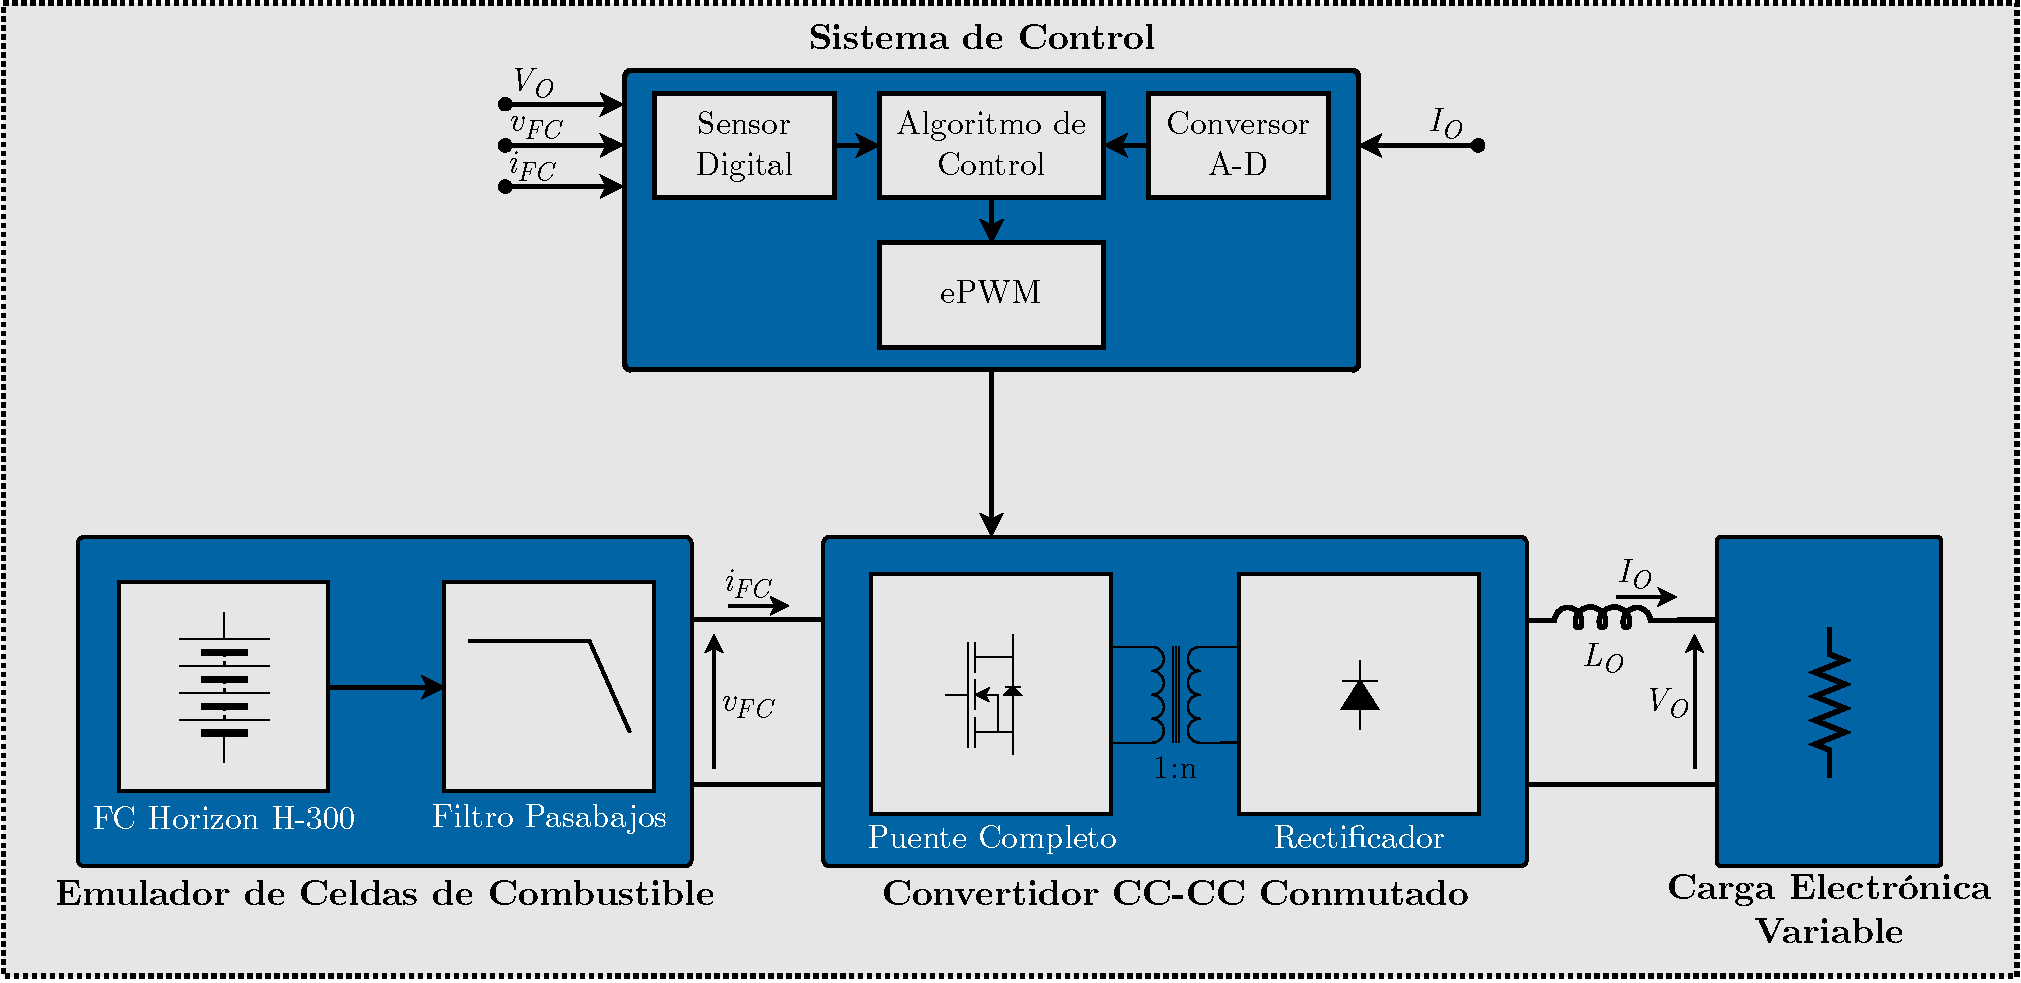
\includegraphics[scale=0.4]{Imagenes/Plataforma Experimental.pdf}
    \caption{Diagrama de la plataforma experimental de evaluación, con sus cuatro bloques principales.}
    \label{diag_plataforma}
\end{figure}

Esta plataforma, con sus distintos bloques, se encarga de evaluar la \textit{performance} de celdas de combustible conectadas a un sistema híbrido de generación. Con este fin, un emulador de celdas de combustible toma el puesto de celdas de combustible reales, y una carga electrónica variable se utiliza para simular cualquier tipo de condiciones de carga que se deseen en el bus de CC. Para poder conectar el emulador a la carga, se debe implementar un subsistema (Conversor CC-CC Conmutado) que adapte los niveles de tensión de salida del emulador de celdas a la tensión fija de salida en la carga, adicionando un módulo de control que monitorea los estados del conversor, y los controla mediante los disparos de las llaves del puente completo.\\

El principal objetivo de este proyecto es el diseño e implementación de la etapa de adaptación de tensión (es decir, el conversor con su sistema de control), pero se hace un estudio detallado de todas los componentes de la plataforma, de manera de obtener un entendimiento más completo de todo el sistema. Por esta razón, a continuación se hace un análisis en profundidad de cada una de las partes individuales, comenzando por el emulador de celdas de combustible.\\

\subsection{Emulador de Celdas de Combustible}

Lorem ipsum dolor sit amet, consectetur adipiscing elit, sed do eiusmod tempor incididunt ut labore et dolore magna aliqua. Ut enim ad minim veniam, quis nostrud exercitation ullamco laboris nisi ut aliquip ex ea commodo consequat. Duis aute irure dolor in reprehenderit in voluptate velit esse cillum dolore eu fugiat nulla pariatur. Excepteur sint occaecat cupidatat non proident, sunt in culpa qui officia deserunt mollit anim id est laborum.\\